\chapter{ Stay Tuned for next chapters!}
\begin{tikzpicture}
  \matrix (m) [matrix of math nodes, row sep=5em, column sep=5em]
    { 0 & A  & B  & C  & 0 \\
      0 & A' & B' & C' & 0 \\ };
  { [start chain] \chainin (m-1-1);
    \chainin (m-1-2);
    { [start branch=A] \chainin (m-2-2)
        [join={node[right,labeled] {\eta_1}}];}
    \chainin (m-1-3) [join={node[above,labeled] {\varphi}}];
    { [start branch=B] \chainin (m-2-3)
        [join={node[right,labeled] {\eta_2}}];}
    \chainin (m-1-4) [join={node[above,labeled] {\psi}}];
    { [start branch=C] \chainin (m-2-4)
        [join={node[right,labeled] {\eta_3}}];}
    \chainin (m-1-5); }
  { [start chain] \chainin (m-2-1);
    \chainin (m-2-2);
    \chainin (m-2-3) [join={node[above,labeled] {\varphi'}}];
    \chainin (m-2-4) [join={node[above,labeled] {\psi'}}];
    \chainin (m-2-5); }
\end{tikzpicture}



\begin{tikzcd}
A \arrow[rd] \arrow[r, "\phi"] & B \arrow[d] \\
& C
\end{tikzcd} 

      
\begin{tikzcd}[row sep=small]
& B \arrow[dd] \\
A \arrow[ur] \arrow[dr] & \\
& C
\end{tikzcd}

\begin{tikzcd}[column sep=small]
& A \arrow[dl] \arrow[dr] & \\
B \arrow{rr} & & C
\end{tikzcd}

\begin{tikzcd}
A \arrow[to=Z, red] \arrow[to=2-2, blue]
& B \\
|[alias=Z]| C
& D
\arrow[from=ul, to=1-2, purple]
\end{tikzcd}

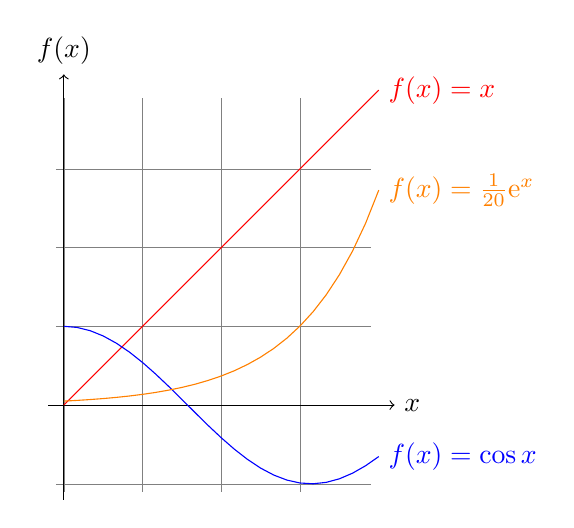
\begin{tikzpicture}[domain=0:4]\draw[very thin,color=gray] (-0.1,-1.1) grid (3.9,3.9);\draw[->] (-0.2,0) -- (4.2,0) node[right] {$x$};\draw[->] (0,-1.2) -- (0,4.2) node[above] {$f(x)$};\draw[color=red] plot (\x,\x) node[right] {$f(x) =x$};\draw[color=blue] plot (\x,{cos(\x r)}) node[right] {$f(x) = \cos x$};\draw[color=orange] plot (\x,{0.05*exp(\x)}) node[right] {$f(x) = \frac{1}{20} \mathrm e^x$};\end{tikzpicture} 